\section{Datenbank-Definitionssprachen}
\label{sec:definitionssprachen}

\textbf{Gewinnung der Konventionen}
\begin{items}
	\item Beschränkte Anwendungswelt (= Miniwelt, relevanter Weltausschnitt, Diskursbereich)
	\item \underline{Daten}: Modelle (gedankliche Abstraktionen) der Miniwelt
	\item \underline{Datenbasiskonsistenz}: Datenbasis ist bedeutungstreu, wenn ihre Elemente Modelle einer gegebenen Miniwelt sind (schärfste Konsistenzforderung)
\end{items}

\textbf{Datenbankentwurf -- Phasenmodell}
\begin{figure}[H]\centering\label{Phasenmodell}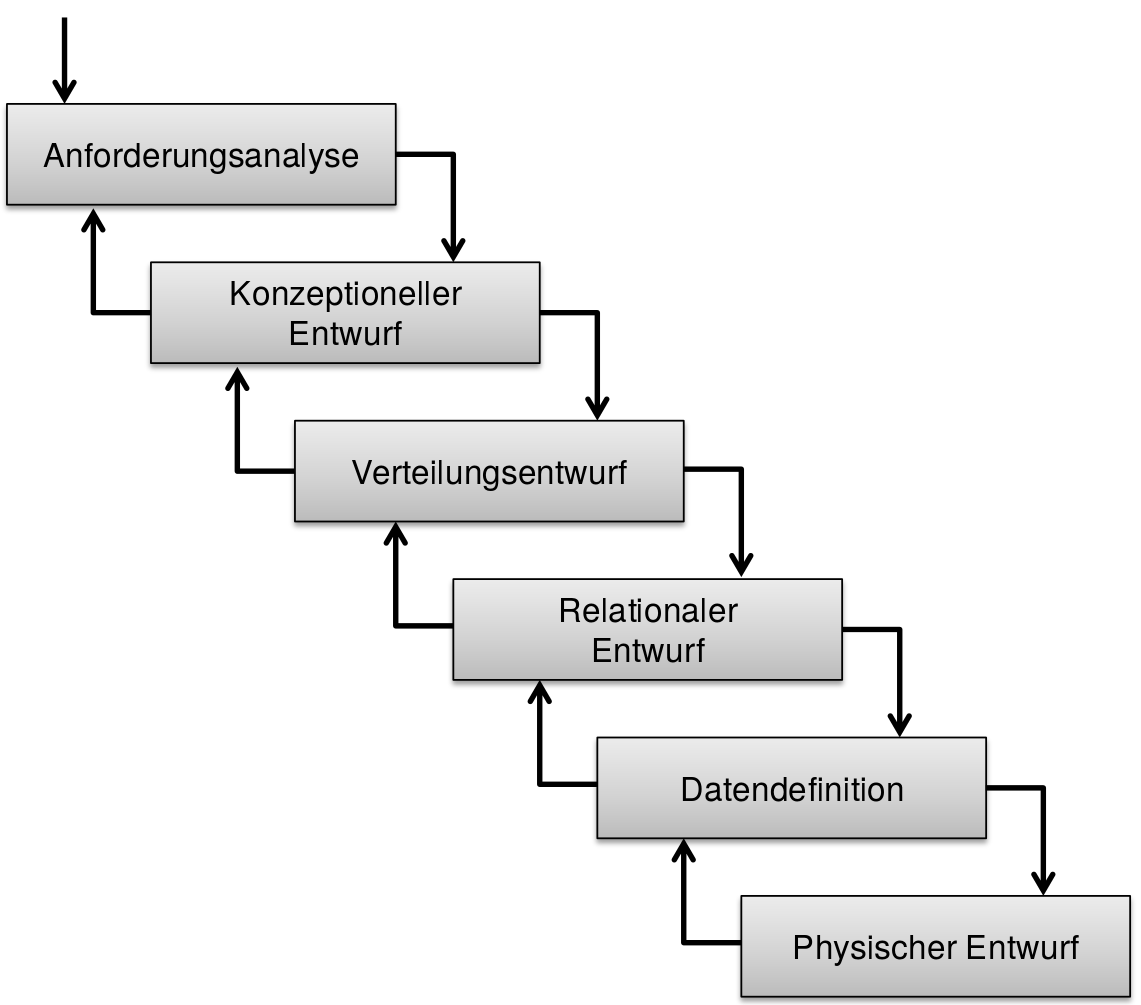
\includegraphics[width=0.33\textwidth]{Phasenmodell}\end{figure}

\textbf{Datenbankentwurf -- Modellierung}
\begin{items}
	\item Ausschnitt der Wirklichkeit mit Schema beschreiben
	\item Typen = Struktur der Entitäten
	\item Welche Konsistenzbedingungen sind sinnvoll?
\end{items}